% by Mirella M. Moro; version: January/18/2012 @ 04:16pm
% -- 01/18/2012: more discussion on SBBD + JIDM; overall revision
% -- 09/03/2010: bib file with names for proceedings and journals; cls with shrinked {received}
% -- 08/27/2010: appendix, table example, more explanation within comments, editors' data

\documentclass[jidm,a4paper]{jidm} % NOTE: JIDM is published on A4 paper
\usepackage{graphicx,url}  % for using figures and url format
\usepackage[T1]{fontenc}   % avoids warnings such as "LaTeX Font Warning: Font shape 'OMS/cmtt/m/n' undefined"

%\usepackage{cite} % NOTE: do **not** include this package because it conflicts with jidm.bst

% Standard definitions
\newtheorem{theorem}{Theorem}[section]
\newtheorem{conjecture}[theorem]{Conjecture}
\newtheorem{corollary}[theorem]{Corollary}
\newtheorem{proposition}[theorem]{Proposition}
\newtheorem{lemma}[theorem]{Lemma}
\newdef{definition}[theorem]{Definition}
\newdef{remark}[theorem]{Remark}

% New environment definition
\newenvironment{latexcode}
{\ttfamily\vspace{0.1in}\setlength{\parindent}{18pt}}
{\vspace{0.1in}}

% ALL FIELDS UNTIL BEGIN{document} ARE MANDATORY

% The following data (volume, number and page) are given by the editors prior to publishing your article
\jidmVolume{5}
\jidmNumber{1}
\jidmYear{14}
\jidmMonth{June}
\setcounter{page}{1}


% Includes headers with simplified name of the authors and article title
\markboth{A.C. Salgado and V. Braganholo}
{JIDM - Journal of Information and Data Management}
%  -> \markboth{}{}
%         takes 2 arguments
%         ex: \markboth{M. M. Moro}{Any article title}


% Title of the article
\title{JIDM - Journal of Information \\ and Data Management\footnote{The original version of this template, which was used up to volume 3, was created by Alberto Laender and Mirella Moro}}


% List of authors
%IF THERE ARE TWO or more institutions, please use:
%\author{Name of Author1\inst{1}, Name of Author2\inst{2}, Name of Author3\inst{2}}
\author{Ana Carolina Salgado\inst{1}, Vanessa Braganholo\inst{2}}


%Affiliation and email
\institute{Universidade Federal de Pernambuco, Brazil \\ \email{acs@cin.ufpe.br}
\and Universidade Federal Fluminense, Brazil \\ \email{vanessa@ic.uff.br}
% IF THERE IS ANOTHER INSTITUTION:
%\and Name_of_the_second_institution \\
%\email{address@whatever.com}
}


% Article abstract - it should be from 100 to 300 words
\begin{abstract}
JIDM is an electronic publication focusing on information and data management in large repositories and document collections. This article introduces the journal, its scope and topics, and the submission process. Finally, it also summarizes information on SBBD, due to its close relation with the symposium.\cite{Baeza-YatesR99}
\end{abstract}


% ACM Computing Classification System categories
\category{H.2}{Database Management}{Miscellaneous} 
\category{H.3}{Information Storage and Retrieval}{Miscellaneous}
\category{I.7}{Document and Text Processing}{Miscellaneous}

% Categories and Descriptors are available at the 1998 ACM Computing Classification System
% http://www.acm.org/about/class/1998/
%  -> \category{}{}{}
%         takes 3 arguments for the Computing Reviews Classification Scheme.
%         ex: \category{D.3.3}{Programming Languages}{Language Constructs and Features}
%                   [data types and structures]
%                   the last argument, in square brackets, is optional.

% Article keywords
\keywords{JIDM, SBBD, template}
%  -> \keywords{} (in alphabetical order \keywords{document processing, sequences,
%                      string searching, subsequences, substrings})


% THE ARTICLE BEGINS
\begin{document}

% This is optional:
\begin{bottomstuff}
% similar to \thanks
% for authors' addresses; research/grant statements
\end{bottomstuff}

\maketitle


% ARTICLE NEW SECTION
\section{Call for Contributions}

JIDM is an electronic publication focusing on information and data management in large repositories and document collections. It relates to different areas from Computer Science, including databases, information retrieval, digital libraries, knowledge discovery, data mining, geographical information systems, among others.

% ARTICLE NEW SUBSECTION
\subsection{Scope and Topics}

JIDM welcomes articles on a full range of research on information and data management, including (but not limited to):

% LIST OF ITEMS
\begin{itemize}
	\item Active Databases 
	\item Access methods and indexing 
	\item Authorization, Privacy and Security 
	\item Concurrency Control and Recovery 
	\item Data Mining and Knowledge Discovery 
	\item Data Semantics 
	\item Data Visualization 
	\item Data Warehousing 
	\item Database Design 
	\item Digital Libraries 
	\item Geographical Information Systems 
	\item Information Integration and Interoperability 
	\item Information Retrieval 
	\item Knowledge Bases 
	\item Mobile Data 
	\item Multidimensional and Temporal Databases 
	\item Multimedia Databases 
	\item Object-Orientation and Databases 
	\item Peer to peer, Parallel and Distributed Databases 
	\item Performance and Benchmarking 
	\item Query Languages and User Interfaces 
	\item Query Processing and Optimization 
	\item Scientific and Statistical Databases 
	\item Semi-structured Databases and XML 
	\item Self-managed and Autonomic Databases 
	\item Spatial Databases 
	\item Stream-based processing and Sensor Databases 
	\item Textual Databases 
	\item Web Databases 
	\item Web Services 
\end{itemize}

\subsection{Types of Submission}

JIDM welcomes \textbf{research} articles that both lay theoretical foundations and provide new insights into the aforementioned areas. JIDM also solicits \textbf{surveys} that should make a contribution to our understanding of related topics from the information and data perspective. Eventually, JIDM may publish \textbf{reports} of meetings and working groups organized to evaluate the future of a given research field. Each article will be reviewed by three different peers. 


\subsection{Submission Instructions}

Research articles should have up to \textbf{12} pages, survey articles up to \textbf{20} pages, and reports up to \textbf{6} pages. The editors should be contacted if more pages are necessary. Articles must be submitted in a PDF file according to the journal format.
Articles should be submitted by JIDM website at: 

\begin{center}
\texttt{http://seer.lcc.ufmg.br/index.php/jidm}
\end{center}



\subsection{Format Instructions}

All camera ready submissions must use LATEX. Thus, we do not provide a MS Word template. The templates for LATEX are available at the associated editor's webpage:

\begin{center}
\url{http://www.ic.uff.br/~vanessa/jidm}
\end{center}

This folder has the following files:

\begin{itemize}
	\item template.pdf
	\item jidm-template.zip
\end{itemize}

where the compacted files have: 

\begin{itemize}
	\item jidmb.bib - an example of bibliography entries
	\item jidm.cls - the latex template class for jidm
	\item jidm.bst - the latex template for bibliography entries
	\item template.tex - an example of tex file (with a figure in \textit{schedule.eps})
\end{itemize}

Prospective authors should take a look at the template.tex for more information on the format, for example: how to add more than one institution to the affiliation and  references to books \cite{Baeza-YatesR99}, book chapters \cite{BorgidaCL09}, conference papers \cite{FerreiraGALV09}, conference papers on book series (e.g., LNCS) \cite{SilvaLC96}, journal articles \cite{LaenderMNM09}, PhD thesis \cite{Moro07} and information published online\footnote{Note: in case the URL refers to a software, dataset source or any other information that does not have a proper author, it is better to include it as a footnote, e.g.: ``Biblioteca Digital Brasileira de Computa\c{c}\~{a}o: http://www.lbd.dcc.ufmg.br/bdbcomp''} \cite{xpath}. The file \textit{jidmb.bib} has examples of how to name conference proceedings and journals. In addition, Appendix A overviews the most important Latex instructions and is a ``must-read'' for authors with little or no experience in Latex, and Appendix B presents the most common errors.

\section{JIDM and SBBD}

SBBD - the Brazilian Symposium on Databases- is the official database event of the Brazilian Computer Society (SBC). It is the largest venue in Latin America for presentation and discussion of research results in the database domain. SBBD joins researchers, students and practitioners, from Brazil and abroad, for discussing problems related to the main topics in modern database technologies. 

From 2010 on, SBBD submission process is integrated with JIDM. 
Each year, SBBD has its own call for papers with specific topics and program committee. Submissions received between \textbf{December} and \textbf{May} are evaluated by SBBD PC members, while the others are evaluated by JIDM reviewers (note that there is a considerable intersection between the two sets of reviewers).

Once SBBD deadline has passed, the submissions go through a first round of revisions and the authors shall receive their reviews by middle \textbf{June}. These reviews may request the submission to be revised and the revised version must be submitted by beginning of \textbf{July} for another review round (the correct dates are published in the SBBD call for papers). The reviews and acceptances for the revised version will be sent to authors by middle \textbf{August}.


\textbf{Very important: All papers published in JIDM must have a presentation in the closest SBBD}, according to the following agenda. All papers accepted by middle August will be published in the October edition and presented at the upcoming SBBD. Papers that are accepted after that date should be published in the February JIDM edition and presented at SBBD in the following year. For example, Figure \ref{fig:schedule} illustrates the regular schedule for JIDM and SBBD, which is also represented in Table \ref{table:schedule} (in order to show how to add figures and tables to your article).


% EXAMPLE OF HOW TO INCLUDE eps FIGURES
\begin{figure}[t] % FIGURES SHOULD BE AT THE TOP [t] OR BOTTOM [b} OF PAGES
\begin{center}	% FIGURES SHOULD BE CENTERED
		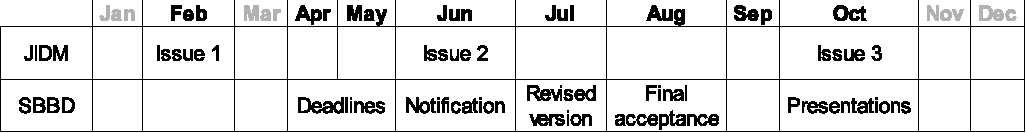
\includegraphics[width=0.9\textwidth]{schedule.pdf} % YOU MAY SHRINK YOUR FIGURE WITH width
	\caption{JIDM and SBBD schedules: as a figure\label{fig:schedule}}	
       % ALWAYS INCLUDE CAPTIONS IN YOUR FIGURES
	 % USE THE CONTENT WITHIN label FOR REFERENCING IT (USE \ref WITHIN THE TEXT)
\end{center}
\end{figure}

Papers submitted to both JIDM and SBBD must not have been simultaneously submitted to any other forum (conference or journal), nor should they have already been published elsewhere.  The acceptance of a paper implies that at least one of its authors will register for the symposium to present it. Submitted papers will be reviewed based on originality, relevance, technical soundness and clarity of presentation.

Full papers must be composed using the JIDM template. Papers exceeding the page limit of the submission type will be automatically rejected without being reviewed by the Program Committee. In addition, all papers must be submitted in PDF format. Formats other than PDF will NOT be accepted. However, exceptionally and upon request, generic postscript might be accepted.



% EXAMPLE OF HOW TO WRITE A TABLE IN LATEX
% DO CHECK http://en.wikibooks.org/wiki/LaTeX/Tables FOR MORE TIPS & TRICKS ON TABLES
\begin{table}[t]% TABLES SHOULD BE AT THE TOP [t] OR BOTTOM [b} OF PAGES
	\caption{JIDM and SBBD schedules: as a table (with different font resources)\label{table:schedule}} 
       % ALWAYS INCLUDE CAPTIONS IN YOUR TABLES
	 % USE THE CONTENT WITHIN label FOR REFERENCING IT (USE \ref WITHIN THE TEXT)

\sffamily % CHANGES THE FONT WITHIN THE TABLE TO sans serif
\begin{center} %TABLES SHOULD BE CENTERED
\begin{tabular}{r|c|c|c|c|c|c|c|c|c|c|c|c|}
	\cline{2-13}  % DRAWS HORIZONTAL LINE FROM 2nd to 13th COLUMNS
	& \rotatebox{90}{Jan } % ROTATES TEXT 90o
	& \rotatebox{90}{Feb} &\rotatebox{90}{Mar} &\rotatebox{90}{Apr} &\rotatebox{90}{May } &\rotatebox{90}{Jun} &\rotatebox{90}{Jul} &\rotatebox{90}{Aug} &\rotatebox{90}{Sep} &\rotatebox{90}{Oct} &\rotatebox{90}{Nov} &\rotatebox{90}{Dec} \\ \hline % DRAWS HORIZONTAL LINE
\multicolumn{1}{|r|}{JIDM} % THIS multicolumn JUST GUARANTEES THE VERTICAL LINE AT THE BEGINNING OF THE COLUMN
& -- & Issue 1 & -- & -- & --                         & Issue 2      & --      & --         & -- & Issue 3 & -- & -- \\ \hline
\multicolumn{1}{|r|}{SBBD} & -- &         & -- & \multicolumn{2}{|c|}{SBBD} % THIS multicolumn MERGES TWO CELLS
& Notification & Revised & Final      & -- & Presentations & -- & -- \\ 
\multicolumn{1}{|r|}{}     &    &         &    & \multicolumn{2}{|c|}{Deadlines} &              & Version & Acceptance &  &  & & \\ \hline
\end{tabular}
\end{center}
\rmfamily % RESTORES TO TIMES, SO THAT CAPTION IS WRITTEN PROPERLY
\end{table}


% INCLUDE BIBLIOGRAPHY WHICH MUST FOLLOW jidm.bst TEMPLATE
\bibliographystyle{jidm}
\bibliography{jidmb}
% For information on how to write bibliography entries, 
% see file jidmb.bib





\end{document}
